\chapter{GIỚI THIỆU ĐỀ TÀI}

	\fontsize{12pt}{7pt}\selectfont
	\noindent\textit{Chương này sẽ giới thiệu một cách sơ lược về đề tài và cấu trúc của Luận Văn Tốt Nghiệp. Phần đầu của chương sẽ nêu lên tầm quan trọng và ứng dụng của chuẩn SCORM đối với nhu cầu thực tế hiện tại, hệ thống được lựa chọn để phát triển và các chức năng được hiện thực trong phạm vi giới hạn của Luận Văn này. Mục tiếp theo sẽ trình bày cấu trúc của Luận Văn Tốt Nghiệp.}

\section{Tầm quan trọng của đề tài}

	Công nghệ thông tin đang là một lĩnh vực quan trọng của xã hội, vì những ứng dụng thực tế của ngành công nghệ thông tin ngày càng trở nên thiết thực và hữu ích.  Như việc ứng dụng công cụ khai phá dữ liệu vào thương mại điện tử để nắm bắt nhu cầu khách hàng, ứng dụng các mô hình học máy, học sâu vào nhận diện ảnh y khoa, dự báo dòng chảy sông,... Đối với lĩnh vực giáo dục có thể kể đến một ứng dụng rất gần gũi là E-Learning - hệ thống học tập online thông qua việc sử dụng Internet. E-Learning đã cải thiện hoàn toàn hệ thống học tập truyền thống.\\

	Nội dung được hiển thị và trình bày trên E-Learning rất đa dạng và phong phú với nhiều hình thức khác nhau. Các nội dung trên E-Learning có thể ở dạng văn bản, hình ảnh hay video, bài Quiz, các bài kiểm tra với nhiều hình thức khác nhau như câu hỏi trắc nghiệm, tự luận hay điền khuyết,... Người soạn thảo có thể dùng một công cụ biên soạn (Authoring Tool) để xây dựng một bài giảng điện tử, kết hợp nhiều hình thức này với nhau để tạo nên một bài giảng có chất lượng, nội dung phong phú và tránh gây nhàm chán cho người học.\\
	
	Để thực hiện một bài giảng điện tử thì cần phải có hai nhóm công cụ là công cụ để xây dựng bài giảng và công cụ để hiển thị bài giảng. Công cụ xây dựng bài giảng là công cụ giúp người soạn thảo có thể tạo bài giảng và xây dựng nội dung cho bài học. Công cụ để hiển thị bài giảng sẽ hiển thị những nội dung của bài học mà người soạn thảo đã xây dựng cho bài giảng, giúp người học có thể tương tác với những nội dung này.
	
	\begin{center}
		\begin{figure}[htp]
			\begin{center}
				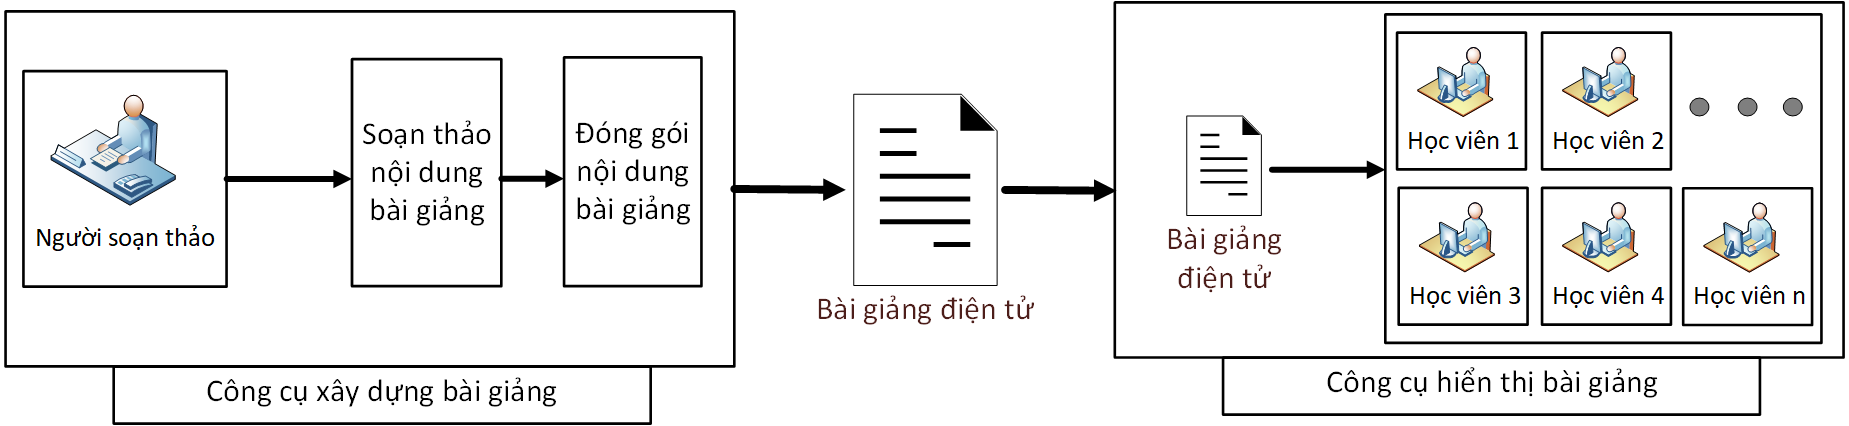
\includegraphics[width=16cm]{Chapter1/Pictures/picture11.png}
			\end{center}
			\caption{Mối quan hệ giữa công cụ xây dựng và hiển thị bài giảng}
			\label{picture11}
		\end{figure}
	\end{center}
	
	\newpage
	
	
	Hình \ref{picture11} thể hiện mối quan hệ giữa công cụ xây dựng bài giảng và công cụ hiển thị nội dung bài giảng. Người soạn thảo sẽ sử dụng công cụ xây dựng bài giảng để tạo bài giảng, xây dựng nội dung cho bài giảng và đóng gói các nội dung này. Sau đó công cụ hiển thị bài giảng sẽ hiển thị nội dung của bài giảng này và giúp người học có thể tương tác với những nội dung của nó.\\
	
	Để hai công cụ này có thể làm việc được với nhau cần có một chuẩn dữ liệu chung, tương thích với cả hai công cụ này. Khi đó các dữ liệu trao đổi giữa hai công cụ này phải tương tác được với nhau, từ đó phát sinh nhu cầu cần có một chuẩn đóng gói dữ liệu giúp hỗ trợ cho việc tương tác giữa hai công cụ này. Có rất nhiều chuẩn đóng gói hiện nay hỗ trợ vấn đề này, trong đó SCORM là một chuẩn như vậy. Chuẩn SCORM là một chuẩn đóng gói bài giảng E-Learning phổ biến nhất hiện nay, được phần lớn các tổ chức sử dụng và chi tiết về chuẩn SCORM sẽ được trình bày trong chương tiếp theo.\\
	
	
	Trong giai đoạn Đề Cương Luận Văn Tốt Nghiệp, nhóm đã tiến hành khảo sát một số SCORM Builder (công cụ soạn thảo có hỗ trợ chuẩn SCORM). Một số SCORM Builder được thương mại hóa như Lectora Inspire 17, Story Line 3, Adobe Presenter,... có độ ổn định cao, cung cấp môi trường soạn thảo đa dạng, tạo được nhiều nội dung tương tác cao với người học và khai thác hoàn toàn thế mạnh của chuẩn SCORM hiện tại. Tuy nhiên, các công cụ thương mại này thường có giá thành rất cao và không có mã nguồn để tham khảo. Bên cạnh đó cũng có một số SCORM Builder có mã nguồn mở như eXe, LAMS, Reload Editor,... Các SCORM Builder có mã nguồn mở cũng có hỗ trợ chuẩn SCORM, cung cấp môi trường soạn thảo,... nhưng các chức năng của chúng vẫn còn hạn chế, chưa khai thác được hết sức mạnh của chuẩn SCORM.\\
	
	
	eXe là một trong số các SCORM Builder có mã nguồn mở hiện nay. eXe hỗ trợ trình soạn thảo có giao diện thân thiện với người dùng, dễ sử dụng, hỗ trợ tạo nội dung bài giảng bằng nhiều hình thức khác nhau như văn bản, hình ảnh hay video,... nó cũng hỗ trợ cho việc tạo bài kiểm tra với nhiều hình thức như câu hỏi trắc nghiệm có nhiều lựa chọn, câu hỏi trắc nghiệm một lựa chọn, điền khuyết,... Tuy nhiên hiện nay chức năng của nó vẫn còn hạn chế, thua xa những SCORM Builder được thương mại hóa khác. eXe giúp người soạn thảo tạo nội dung các bài học, nhưng các bài học này không được quy định thứ tự học, người học có thể ngay lập tức vào học bất kỳ bài học nào có trong bài giảng, điều này sẽ không đảm bảo khả năng tiếp thu của người học. eXe cũng hỗ trợ cho việc tạo bài kiểm tra, nhưng các câu hỏi của bài kiểm tra không có sự phân loại, vị trí các câu hỏi của bài kiểm tra là cố định, điều này sẽ không đảm bảo chất lượng của một buổi kiểm tra vì mọi học viên đều làm các bài kiểm tra có nội dung y hệt nhau.\\
	
	Do đó eXe được nhóm lựa chọn để mở rộng thêm một số chức năng. Chức năng thứ nhất là cho phép người soạn thảo có thể thiết lập thứ tự của các bài học, đưa ra một lộ trình cụ thể cho người học và đảm bảo người học có thể tiếp thu đầy đủ kiến thức của một bài giảng. Chức năng thứ hai là thiết kế một công cụ tạo bài kiểm tra tổng hợp, các câu hỏi trong bài kiểm tra tổng hợp này sẽ có khả năng phân loại độ khó, cuối cùng là vị trí các câu hỏi cũng như câu trả lời của bài kiểm tra này có thể thay đổi được thứ tự ở mỗi lần người học thực hiện. Chi tiết các chức năng được mở rộng sẽ được trình bày ở phần sau.
	
\section{Đề tài luận văn tốt nghiệp}
\subsection{Chức năng điều khiển có điều kiện}

	Hiện tại eXe chỉ hỗ trợ xây dựng bài giảng theo dạng tự do, không có điều kiện. Các bài học trong bài giảng này sẽ không có quy định trình tự học, người học khi bắt đầu tham gia bài giảng có thể ngay lập tức học bất cứ bài học nào có trong bài giảng, kể cả bài cuối cùng mà không cần quan tâm có cần phải học bài nào trước đó hay không. Điều này sẽ không đảm bảo về khả năng tiếp thu kiến thức của người học.
	
		\begin{center}
	\begin{figure}[htp]
		\begin{center}
			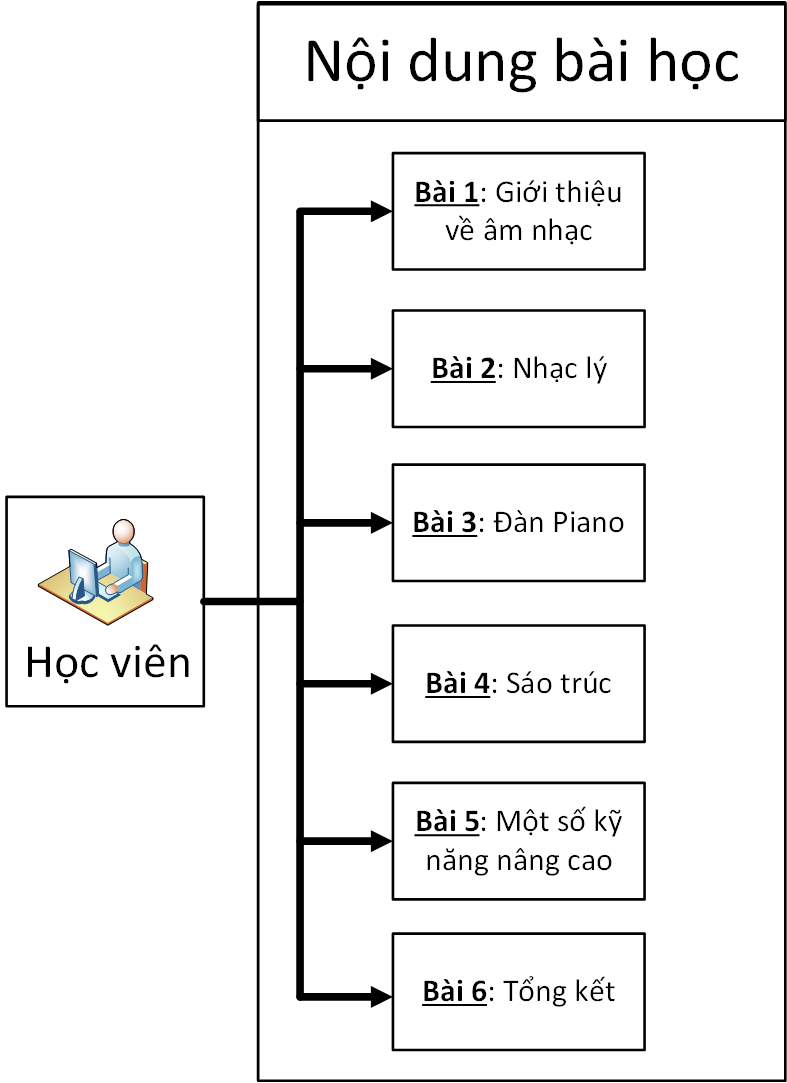
\includegraphics[width=6cm]{Chapter1/Pictures/picture12.png}
		\end{center}
		\caption{Mô hình bài giảng hiện tại của eXe}
		\label{picture13}
	\end{figure}
\end{center}


	
	Hình 1.2 thể hiện ví dụ của mô hình này, khi bắt đầu một bài học, người học có thể di chuyển vào bất cứ bài nào trong một khóa học mà không gặp bất cứ ràng buộc nào. Theo như ví dụ ở hình 1.2 thì người học có thể ngay lập tức học \textbf{Bài 6: Tổng kết}, việc này sẽ ảnh hưởng đến thời gian và hiệu suất học tập của người học, vì nếu như chưa trang bị đủ kiến thức của những bài trước mà lại lựa chọn ngay vào học bài tổng hợp nằm ở cuối cùng thì sẽ không đảm bảo cho việc tiếp thu đầy đủ kiến thức của khóa học.\\
	
	Về mặt chuyên môn, người học cần phải học các bài theo một trình tự khoa học. Trước khi vào học "Bài 2: Nhạc Lý", người học ít nhất cần phải học "Bài 1: Giới thiệu về âm nhạc" trước đó, sau đó "Bài 3: Đàn Piano" phải được học sau "Bài 2: Nhạc lý" vì người học cần phải có kiến thức về nhạc lý trước đó mới có thể học nhạc cụ,... Tuy nhiên eXe chưa hỗ trợ cho việc thiết kế mô hình này. Hình 1.3 thể hiện các bài học được quy định theo một lộ trình cụ thể.
	

	
		\begin{center}
		\begin{figure}[htp]
			\begin{center}
				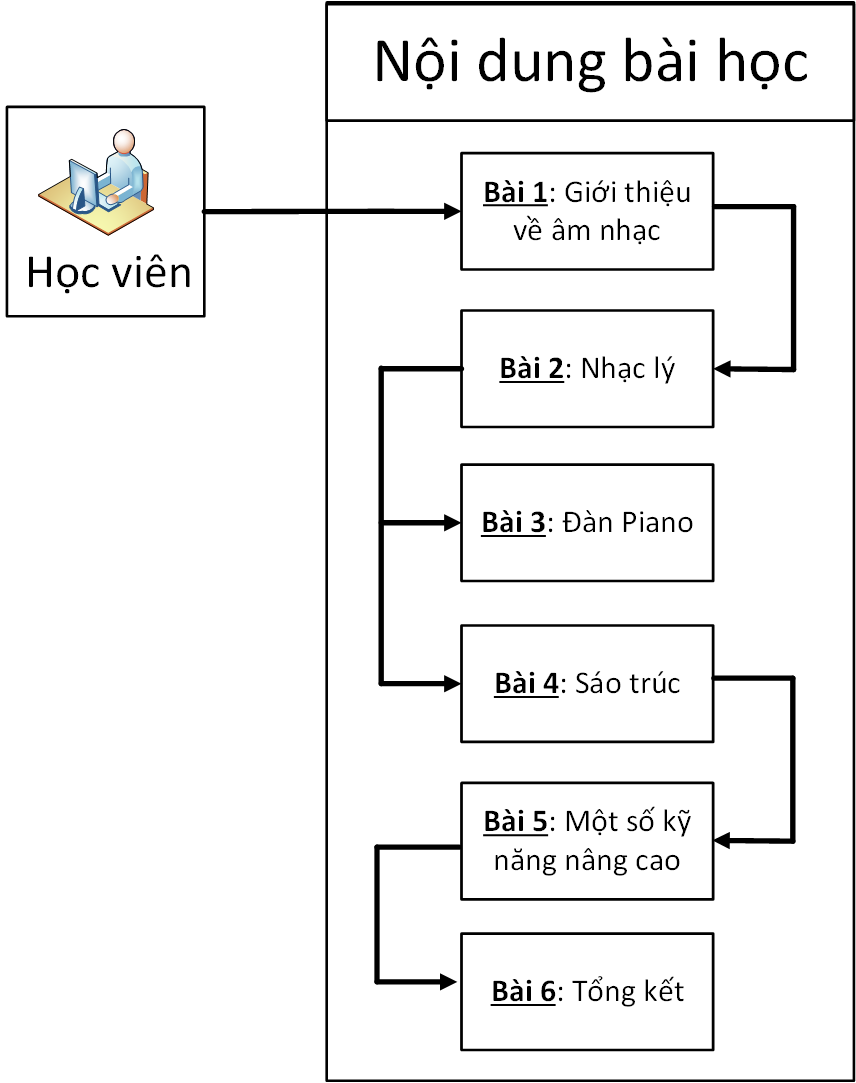
\includegraphics[width=6cm]{Chapter1/Pictures/picture13.png}
			\end{center}
			\caption{Các bài học có thứ tự}
			\label{picture12}
		\end{figure}
	\end{center}
	\newpage
	
	Chức năng điều khiển có điều kiện sẽ giúp người soạn thảo có thể xây dựng bài học như mô hình trên. Chức năng này giúp người soạn thảo có thể thiết lập điều kiện ở mỗi bài, giúp đưa ra một lộ trình học cụ thể. Điều kiện bao gồm tiền điều kiện và hậu điều kiện. Tiền điều kiện là điều kiện mà người học cần thỏa mãn để được vào học một bài học, tiền điều kiện của 1 bài học là bài học mà người học cần phải hoàn thành (thỏa mãn hậu điều kiện) trước khi vào nội dung của bài học này. Hậu điều kiện là điều kiện xác nhận người học đã hoàn thành bài học này, hậu điều kiện có thể là thời gian tối thiểu mà người học phải bỏ ra cho một bài học hoặc phải đạt một số bài kiểm tra nào đó trong bài học do người biên soạn quy định. Sau đây là ví dụ giúp người đọc dễ hình dung hơn.
	
		\begin{center}
		\begin{figure}[htp]
			\begin{center}
				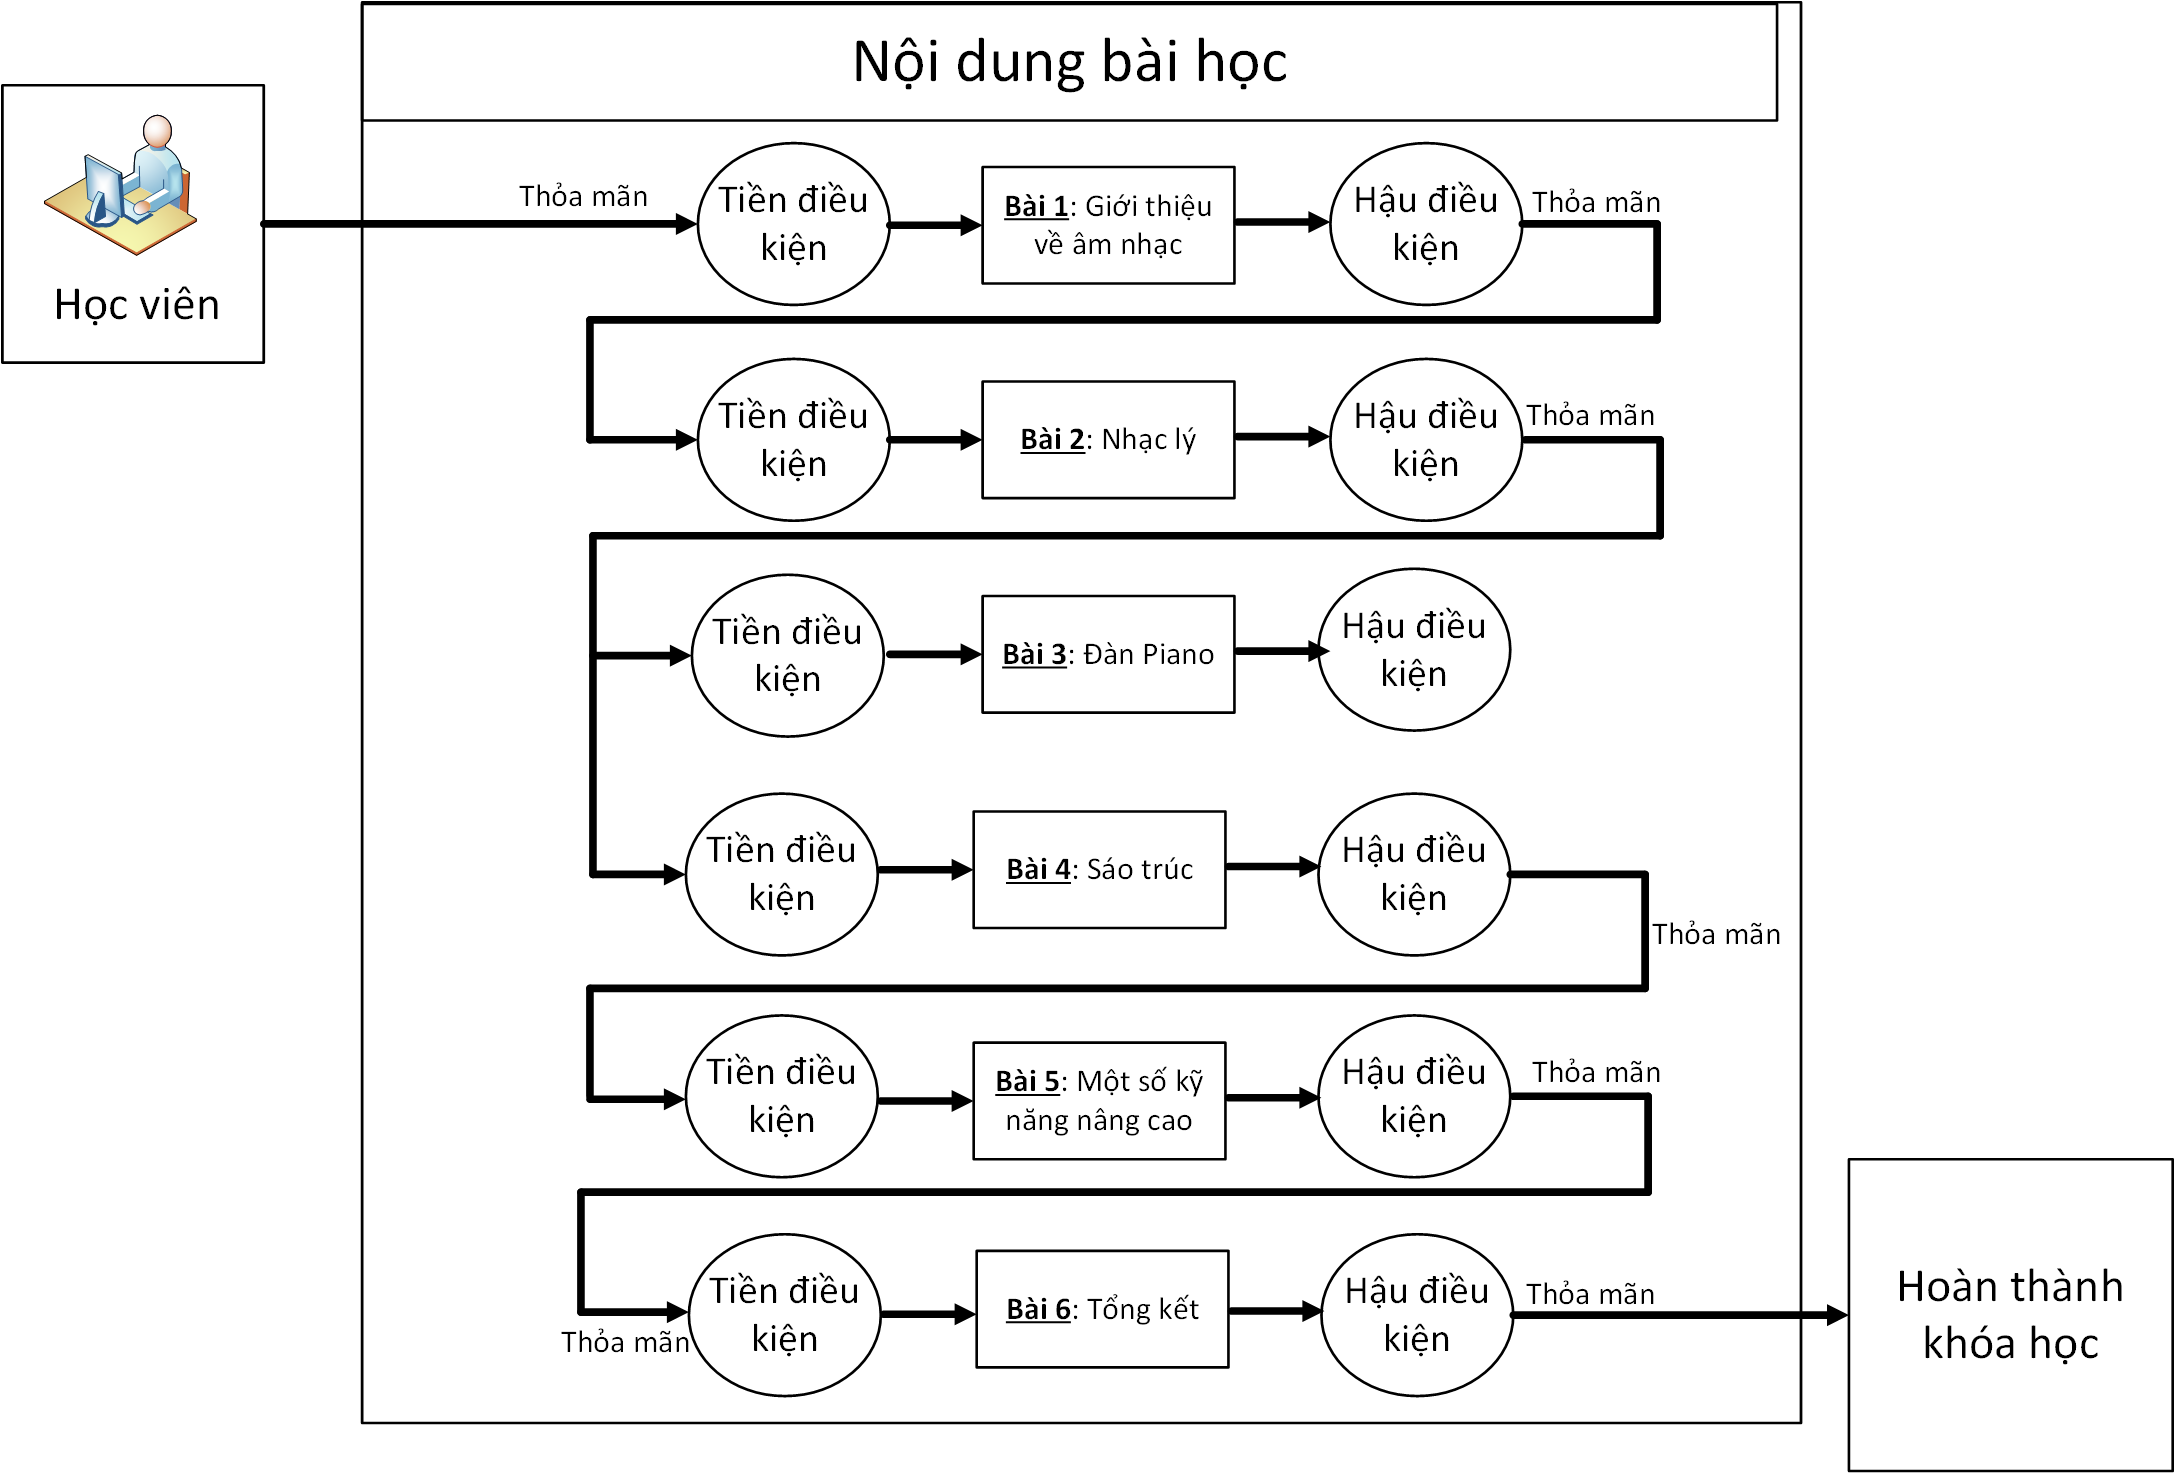
\includegraphics[width=16cm]{Chapter1/Pictures/picture14.png}
			\end{center}
			\caption{Mô hình điều khiển có điều kiện}
			\label{refpicture13}
		\end{figure}
	\end{center}


	Hình 1.4 thể hiện ví dụ một mô hình điều khiển có điều kiện, ở mỗi bài học đều được thiết lập tiền điều kiện và hậu điều kiện tương ứng. Đầu tiên học viên sẽ học "Bài 1: Giới thiệu về âm nhạc", vì đây là bài đầu tiên của khóa học nên sẽ không cần tiền điều kiện. Tiếp theo học viên muốn học "Bài 2: Nhạc lý" thì học viên cần phải thỏa mãn tiền điều kiện của Bài 2 này, tức hậu điều kiện của Bài 1, hậu điều kiện của Bài 1 có thể là thời gian phải bỏ ra hoặc bài kiểm tra cần đạt tùy theo thiết lập của người soạn thảo. Sau khi hoàn thành Bài 2, học viên có thể lựa chọn tiếp tục học "Bài 3: Đàn Piano" hoặc "Bài 4: Sáo trúc", vì nội dung của hai bài này độc lập với nhau. Sau khi hoàn thành "Bài 4: Sáo trúc" thì học viên có thể tiếp tục học "Bài 5: Một số kỹ năng nâng cao" và cuối cùng là "Bài 6: Tổng kết".
	
	
	
	\newpage
	
\subsection{Chức năng tổng hợp câu hỏi và tạo bài kiểm tra}
	
	Trong việc thiết kế một bài giảng điện tử, nhu cầu kiểm tra kiến thức của người học sau mỗi bài học là rất cần thiết. Qua đó có thể biết được người học đã tiếp thu được bao nhiêu kiến thức do người soạn thảo trình bày trong bài học. Do đó trong các SCORM Builder thường có một công cụ cung cấp chức năng soạn thảo câu hỏi, tạo bài kiểm tra cho người biên soạn.\\

	SCORM Quiz là một trong số các công cụ kiểm tra được thiết kế sẵn trong eXe Learning. Đây là một công cụ dùng để tạo bài kiểm tra ở dạng trắc nghiệm. Người soạn thảo có thể thiết lập nhiều câu trả lời trong một câu hỏi, mỗi câu hỏi có một đáp án đúng. Người soạn thảo cũng có thể thiếp lập tỉ lệ đạt cho mỗi SCORM Quiz tùy vào độ khó của bài kiểm tra này. Tuy nhiên bên cạnh đó SCORM vẫn còn rất nhiều nhược điểm.\\
	
	SCORM Quiz hiện tại đang có ba nhược điểm chính. Nhược điểm đầu tiên là trong thiết kế ban đầu của SCORM Quiz, người biên soạn chỉ có thể thiết lập một SCORM Quiz cho mỗi bài học, điều này gây khó khăn cho người biên soạn khi muốn có nhiều SCORM Quiz trong cùng một bài học, giúp đề kiểm tra đa dạng hơn. Nhược điểm thứ hai là không có thuộc tính phân loại cho các câu hỏi, điều này gây khó khăn cho người biên soạn khi cần soạn một đề kiểm tra phù hợp với những yêu cầu khác nhau về các số lượng câu hỏi khó, trung bình hay dễ. Nhược điểm thứ ba là các câu hỏi được trình bày ra cho người học là cố định, không thể thay đổi được vị trí câu hỏi cũng như vị trí câu trả lời, có nghĩa là nhiều người học sẽ thấy và làm những câu hỏi tương tự nhau khi thực hiện bài Quiz.\\
	
	Cần khắc phục những nhược điểm trên của SCORM Quiz, phát triển một công cụ mới có khả năng tổng hợp câu hỏi và tạo bài kiểm tra, SCORM Test là tên của công cụ này. SCORM Test giúp người soạn thảo có thể phân loại câu hỏi bằng cách thiết lập mức độ khó dễ cho từng câu hỏi, cho phép người soạn thảo cấu hình bài kiểm tra bằng cách lựa chọn số câu hỏi với các mức độ khó, trung bình hay dễ sẽ xuất hiện trong bài kiểm tra này, cuối cùng sẽ tổng hợp các câu hỏi này lại và tự động sinh bài kiểm tra dựa trên các câu hỏi đã được chọn, điều quan trọng là vị trí của các câu hỏi cũng các câu trả lời trong bài kiểm tra phải thay đổi trong mỗi lần học, giúp người học có thể thực hiện bài kiểm tra nhiều lần để ôn tập kiến thức và cho người học biết được số điểm họ làm được sau thi thực hiện xong, giúp người học hiểu về khả năng tiếp thu kiến thức của mình.
	
\begin{center}
	\begin{figure}[htp]
		\begin{center}
			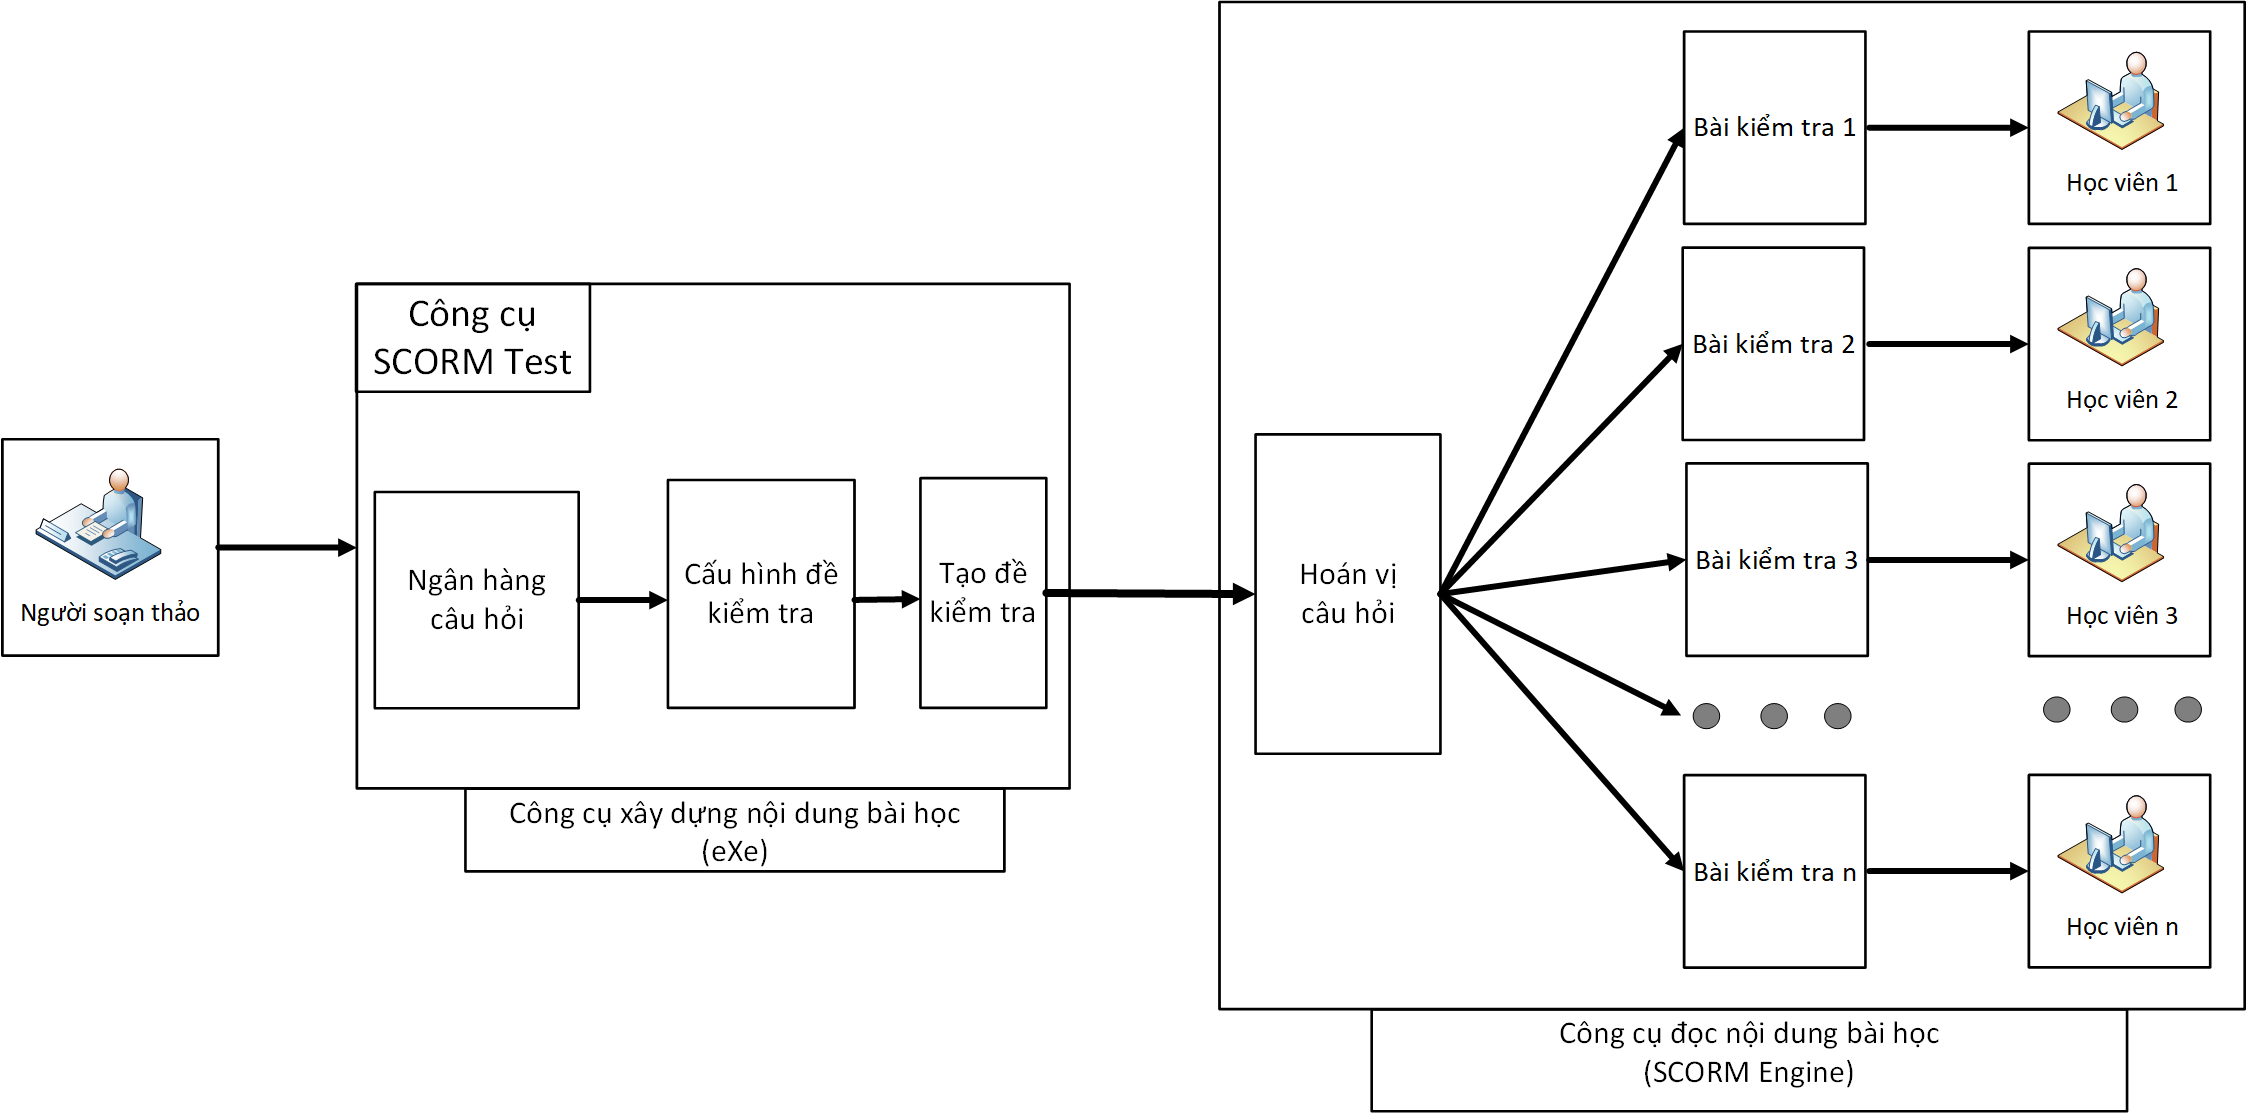
\includegraphics[width=16cm]{Chapter1/Pictures/picture15.png}
		\end{center}
		\caption{Công cụ kiểm tra SCORM Test}
		\label{refpicture14}
	\end{figure}
\end{center}
	
	Hình 1.5 mô tả quá trình sử dụng công cụ SCORM Test. Người soạn thảo sẽ sử dụng công cụ SCORM Test trên eXe, từ ngân hàng đề thi ban đầu, người soạn thảo sẽ tiến hành cấu hình đề thi, chọn ra những câu hỏi theo ý muốn và tạo đề kiểm tra. Sau đó bộ hoán vị câu hỏi bên phía SCORM Engine sẽ đọc bài kiểm tra này và sinh ra những đề kiểm tra tương ứng cho mỗi học viên, thứ tự các câu hỏi cũng như các câu trả lời đều khác nhau đối với mỗi học viên. Điều này sẽ giúp cải thiện chất lượng trong một buổi kiểm tra, các học viên sẽ làm những đề kiểm tra khác nhau và tránh được tình trạng gian lận.

\section{Cấu trúc của báo cáo Luận Văn Tốt Nghiệp}

	Hai chức năng mà nhóm phát triển là thêm các thông tin điều khiển có điều kiện cho các bài học và thiết kế một công cụ giúp tổng hợp câu hỏi và sinh đề kiểm tra. Để hiện thực hai chức năng này, kiến trúc hệ thống của E-Learning, các mô tả của chuẩn SCORM, những kiến thức, công nghệ dùng để phát triển công cụ eXe và kiến trúc hệ thống của eXe đều được tìm hiểu và trình bày ở chương 2. Chương 3 sẽ trình bày chi tiết về cách tích hợp chức năng điều khiển có điều kiện vào công cụ eXe, đưa ra các khái niệm về điều khiển có điều kiện, các mục tiêu, khó khăn và thách thức trong quá trình thực hiện cũng như cơ chế và cách hiện thực chức năng. Nhu cầu cần kiểm tra kiến thức sau bài học, các nhược điểm của bài kiểm tra được tích hợp sẵn trong công cụ eXe cũng như cách thiết kế công cụ để tổng hợp câu hỏi và sinh đề kiểm tra sẽ được trình bày trong chương 4. Chương 5 sẽ trình bày về kiểm thử phần mềm sau khi hiện thực hai chức năng, bao gồm chiến lược kiểm thử, các khó khăn và thách thức trong quá trình kiểm thử cũng như các hướng giải quyết cho các thách thức này và cuối cùng là một số mẫu kiểm tra nhóm đã hiện thực. Phần cuối cùng, chương 6 sẽ đưa ra kết luận về quá trình, tiến độ cũng như kết quả thực hiện đề tài, cuối cùng là các hướng phát triển tiếp theo có thể thực hiện trong tương lai.



